The Bootstrap method is a technique for estimating the variance or median of an estimator based on sampling from the empirical distribution.\\
The aim of this exercise is using Bootstrap method to estimate variance of the estimator(according lecture 10). In this respect, at first we Simulate r  data sets, each with N “observations” sampled form the empirical distribution $F_e$.\\
For each simulated data set, estimate the parameter of interest. This is a bootstrap replicate of the estimate.\\
Finally report the variance among the bootstrap replicates.\\
\\In this exercise we write a subroutine that takes as input a “data” vector of observed values, and which outputs the median as well as the bootstrap estimate of the variance of the median, based on r = 100 bootstrap replicates.\\
\\For testing, we Simulate $n = 200$ Pareto distributed random variates with $\beta = 1$ and $k = 1.05$.\\
Table 7 show the Computation of the mean, the median, and the bootstrap estimate of the variance of the sample median.

\begin{center}
    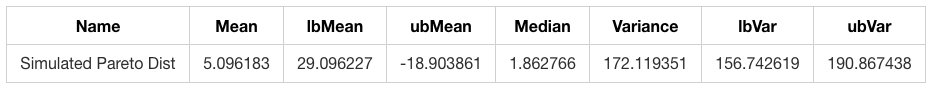
\includegraphics[scale=0.5]{Figures/figure8_2.png}\\
\end{center}\\

\begin{center}
    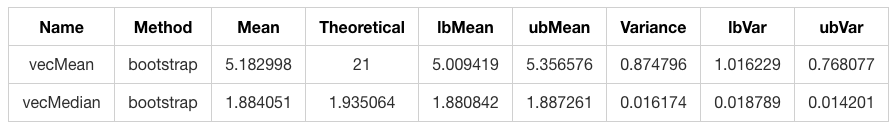
\includegraphics[scale=0.55]{Figures/figure8_1.png}\\
    \figuretitle{Table 9: Bootsrap Result .}
\end{center}\\

From table 9, we can see that the bootstrap method can be used to estimate the sample median. The variance and confidence interval of median can also be calculated, which shows that the estimation is very accurate. For Pareto distribution, it's hard to get the precise mean. Even the variance of the estimated mean from 100 sets is large.